\section*{Overview}


This software, programmed in Python, has a clear objective of providing a new point of view of the source code of Fortran or Python programs. This is aimed to multilayer-based FORTRAN 95 or PYTHON 3.x programs- This means that there are several modules in each layer which call to modules in the lower layers, and which are called from modules in the upper layer. It can handle large amounts of files and directories, so this is suitable for complex projects, like simulations. In python programs it also includes the files of the directory where it is installed. 

It is intended to present different graphs with the main information of the structure of the program. For this is necessary for the program to follow some specifications:

For FORTRAN programs
\begin{itemize}
    \item Every program and module should be in a separated file, whose name should be the same as the module/program name.
    \item If inside a file there is code after an $ end module $ or an $ end program $ line, it will not be read.
    \item This program distinguishes between upper case and lower case, so if there is a call to a module or function, both call and subroutine name should be with identical cases.
    \item Because the same reason as before, all statements and commands proper of FORTRAN should be in lower case.
    \item All files should avoid the BOM Unicode writing, as it could cause reading problems.
\end{itemize}

For PYTHON programs
\begin{itemize}
    \item It only works with any 3.x versions.
    \item All the used packages should be installed.
   \end{itemize}


%\newpage
\section*{Getting started}

Firstly, you will need the software involved in the program. This consist of a folder with following items:

\begin{itemize}
    \item \textbf{"bin" folder} Includes all the program files and source code.
    \item \textbf{"doc" folder} Where this document should be included.
    \item \textbf{"graphs" folder} Where the resulting graphs will be written. This folder is necessary for the program to run, even if it's empty.
    \item \textbf{"excludes.ini"} It is a file which holds the "USES" to be excluded from the graphs. It is read and updated by the program. If you open it with the notebook you can read the last session exclusions (as a python list: $["item1","item2",]$ )
    \item \textbf{"configuration.ini" file} Here, data referred to the previous session is stored. This data is the last directory and main file selected.
    \item \textbf{"graphviz-2.28.0.msi"} It is compulsory to install this software, since it creates the graphs from DOT language. It only takes a few steps.
    \item \textbf{"RUN.bat"} The BAT file that starts the program.% (and shows the interface)
    \item \textbf{Python Portable} For the use of this version, it is necessary to have the "WinPython" folder, which contains the python portable, in the root folder of the program, the folder that contains the program folder.
\end{itemize}

For a successful use of the program you must start with the following steps:

\begin{enumerate}
    \item 
    Before start FortranProgram you should install GraphViz by double-clicking on the "GraphViz.msi" in the folder you have installed FortranProgram. Then follow the instructions.
    \item 
    Once you have installed GraphViz, you can start FortranProgram by double-clicking on the \textbf{"RUN.bat"} file of the main directory where you have installed it, and after a few moments the interface will pop up.
    
\end{enumerate}



\section*{The Interface}




\begin{figure}[H]
    \begin{center}
        \includegraphics[width=1.\linewidth]{\home/images/interface.jpg}
        \caption{The interface}
    \end{center}
\end{figure}



The interface has a very simple and intuitive use. 

First of all, there are four buttons in the lower area. 

\begin{figure}[H]
    \begin{center}
        
\includegraphics[width=1.\linewidth]{\home/images/LowerButtons.jpg}
        \caption{Lower buttons}
    \end{center}
\end{figure}
These are used to select the input directory (\textbf{Select folder...} button), to select the main file where it will start reading (\textbf{Select main file...} button), to start reading  the files (\textbf{Refresh graphs...} button) and modify the \textit{exclusion list} (\textbf{USES excluded}):
\begin{itemize}
    \item \framebox[1.1\width]{\textbf{Select folder...}}   From this button you can select the folder that contains all the $.f90$ or the $.py$ files of source code. In python programs it is not necessary to include the packages installed in the root of python.
    \item \framebox[1.1\width]{\textbf{Select main file...}}   From here you can select the main file of the program which calls to other modules (which are in other files, but contained in the selected folder). You should select the type of file (.f90 or .py) before looking for it in your PC.
    

\item \framebox[1.1\width]{\textbf{Refresh graphs...}}  Refresh the graphs.
\item \framebox[1.1\width]{\textbf{USES excluded}}  In FORTRAN programs: This button opens a window where you can modify the USES (nodes) of the program to be omitted, so these will not appear in the graphs. In PYTHON programs: it opens the same file but in this case there are folders instead of files.f90, which content will be omitted.
\begin{figure}[H]
    \begin{center}
        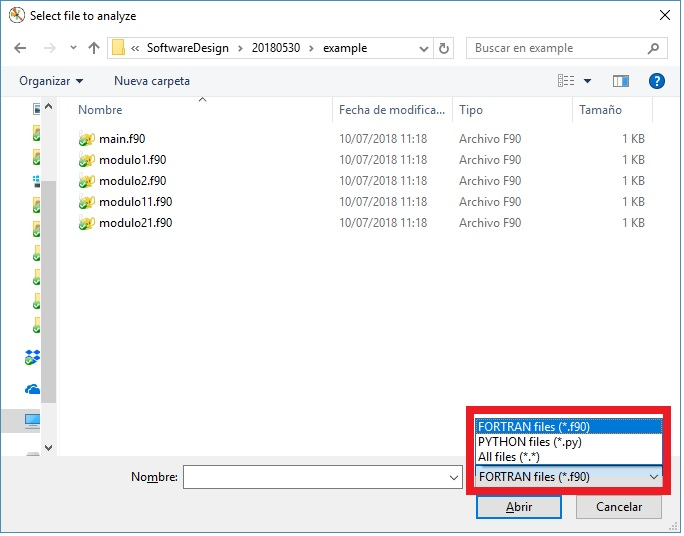
\includegraphics[width=0.9\linewidth]{\home/images/mainfile.jpg}
        \caption{Window that pop ups when you are going to select the main file. At the right lower corner you can select whether to see FORTRAN files or PYTHON files.}
    \end{center}
\end{figure}
\end{itemize}

\textbf{Note that:} The data referred to the selected directory and main file is stored in a file called \textit{configuracion.ini}. So, if you run the program after a previous session, \textit{configuracion.ini} will be read, and you will find that the directory and main file of the previous session is selected. Then, if you wanted to analyze the same directory and folder, you could click on "\textbf{Refresh Graphs...}" directly without selecting directory and folder again.

%\newpage
\newpage
Then, at the upper left corner we have a list of output graphs. After we first refresh the graphs, the graphs will be available. We can choose between a use's graph, a complete use's graph, a type graph, and a complete type graph:


\begin{itemize}
    \item \textbf{Use's graph}
    \item \textbf{Complete use's graph}
    \item \textbf{Type graph} (Only available for fortran programs)
    \item \textbf{Complete type graph} (Only available for fortran programs)
\end{itemize}

These will be explained later

\begin{figure}[H]
    \begin{center}
        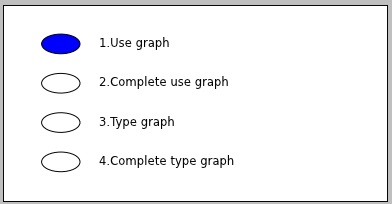
\includegraphics[width=0.4\linewidth]{\home/images/LeftButtons.jpg}
        \caption{List of available graphs. Only the two first are works with python graphs.}
    \end{center}
\end{figure}

The main area, which is in blank at the beginning, is where the graphs are showed. After reading the files, the first of the graphs will be presented here automatically. If there is any type of error in any graph, the graphs will not show up directly, and only by pressing the buttons of the list will pop up the ones successfully made.

Finally in the lower left corner there are some buttons related to the graph handle, which are not relevant for the use of the SoftwareDesign program, as the results are stored in the \textbf{"graphs" folder}. This buttons could be used to zoom or move the graphs in the display area, or to save the selected graph in a specific format.



\newpage

\section*{Graphs}


As we said, the result are four graphs for FORTRAN programs and two graphs for PYTHON programs, which you can see with the buttons of the left in the white area. Apart from that, the graphs are saved in the folder \textit{graphs}, in the same directory as the SoftwareDesign program. 

%\newpage
\begin{figure}[H]
	\begin{center}
		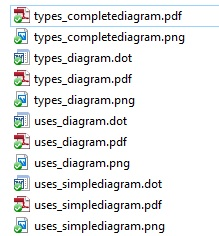
\includegraphics[width=0.4\linewidth]{\home/images/GraphFiles.jpg}
	\end{center}
\end{figure}

Each graph is saved in three different formats: JPG, PDF and DOT. DOT is the lenguage which is used by the GraphViz software, a sub-program that creates the graphs.


\begin{itemize}
    \item \textbf{Use graph:} Files are arranged with main file in the upper layer, followed by the modules in the second layer, which are used with the $ use $ statement by the main file. Down them are the modules used by the modules from the second layer.
    \item \textbf{Complete use graph:} This one is the same as the previous one, but with extra information within the labels. This includes functions, subroutines and types held in each file.
    \item \textbf{Type graph:} Types are arranged as some of them are extended from others located in the same or in other file, or because inside of some of them there are other types as a part of the main. Labels of types are inside square labels that indicates where are they contained. Only for FORTRAN programs.
    \item \textbf{Complete type graph:} This one is the same as the previous one, but is included in the label the part of the code that defines each type. Only for FORTRAN programs.
\end{itemize}

If reached some point it is found that there is a use to a module that isn't found, it will be represented as an elliptic label, instead of a box with rounded corners.

\newpage

\section*{Examples}

This is the result of the analysing the folder "Example", selecting "main.f90" as the main FORTRAN file.

\begin{figure}[H]
    \begin{center}
        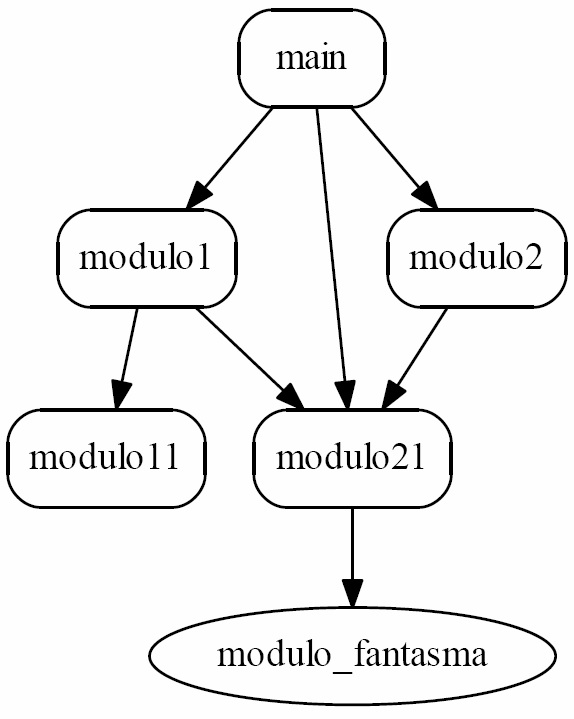
\includegraphics[width=0.3\linewidth]{\home/images/Example1.jpg}
        \caption{Use Graph}
    \end{center}
\end{figure}

\begin{figure}[H]
    \begin{center}
        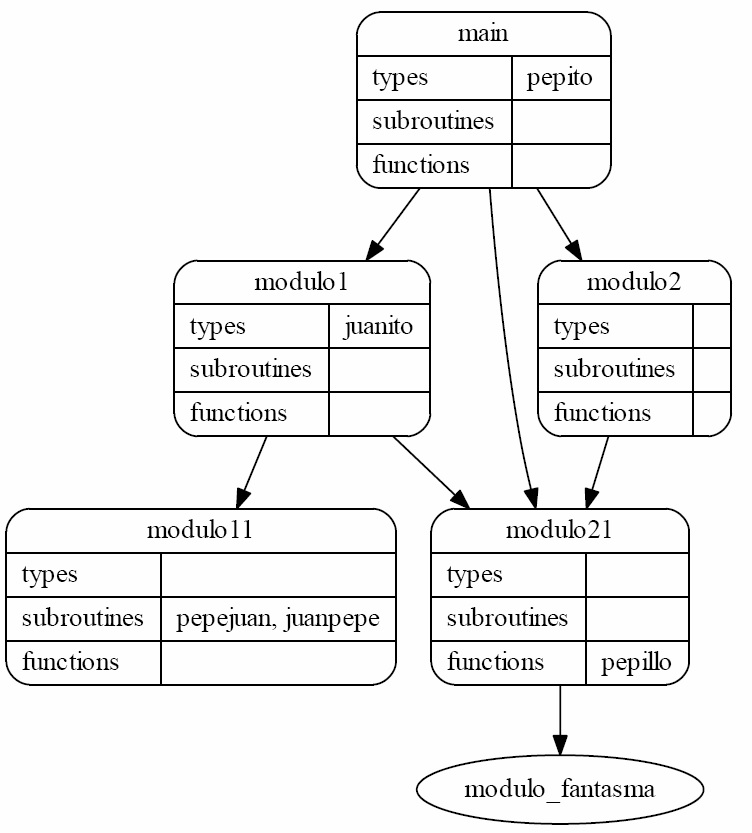
\includegraphics[width=.55\linewidth]{\home/images/Example2.jpg}
        \caption{Complete Use Graph}
    \end{center}
\end{figure}


\begin{figure}[H]
    \begin{center}
        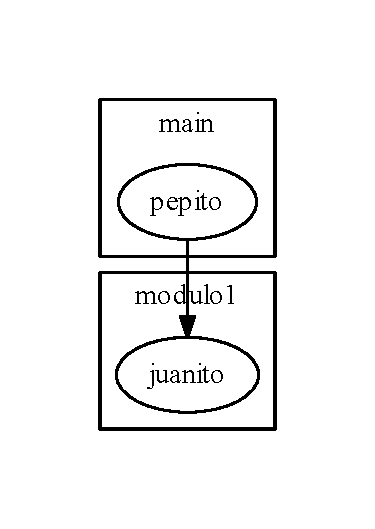
\includegraphics[width=.3\linewidth]{\home/images/Example3.pdf}
        \caption{Type Graph}
    \end{center}
\end{figure}


\begin{figure}[H]
    \begin{center}
        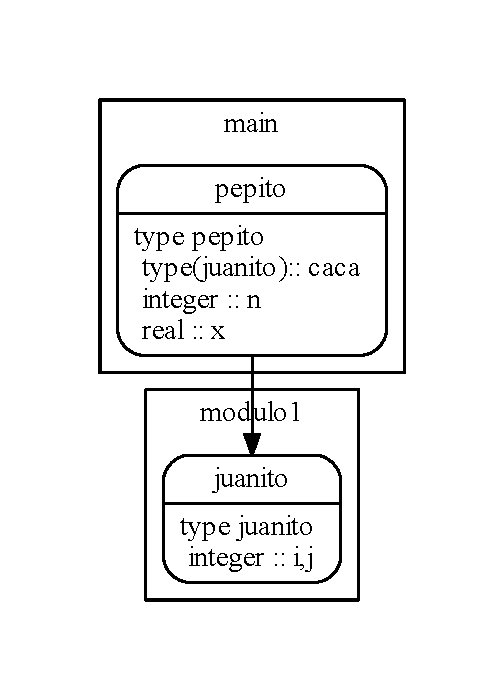
\includegraphics[width=.4\linewidth]{\home/images/Example4.pdf}
        \caption{Complete Type Graph}
    \end{center}
\end{figure}
\newpage

This is the result of the analysing the folder "Example", selecting "main.py" as the main PYTHON file.

\begin{figure}[H]
    \begin{center}
        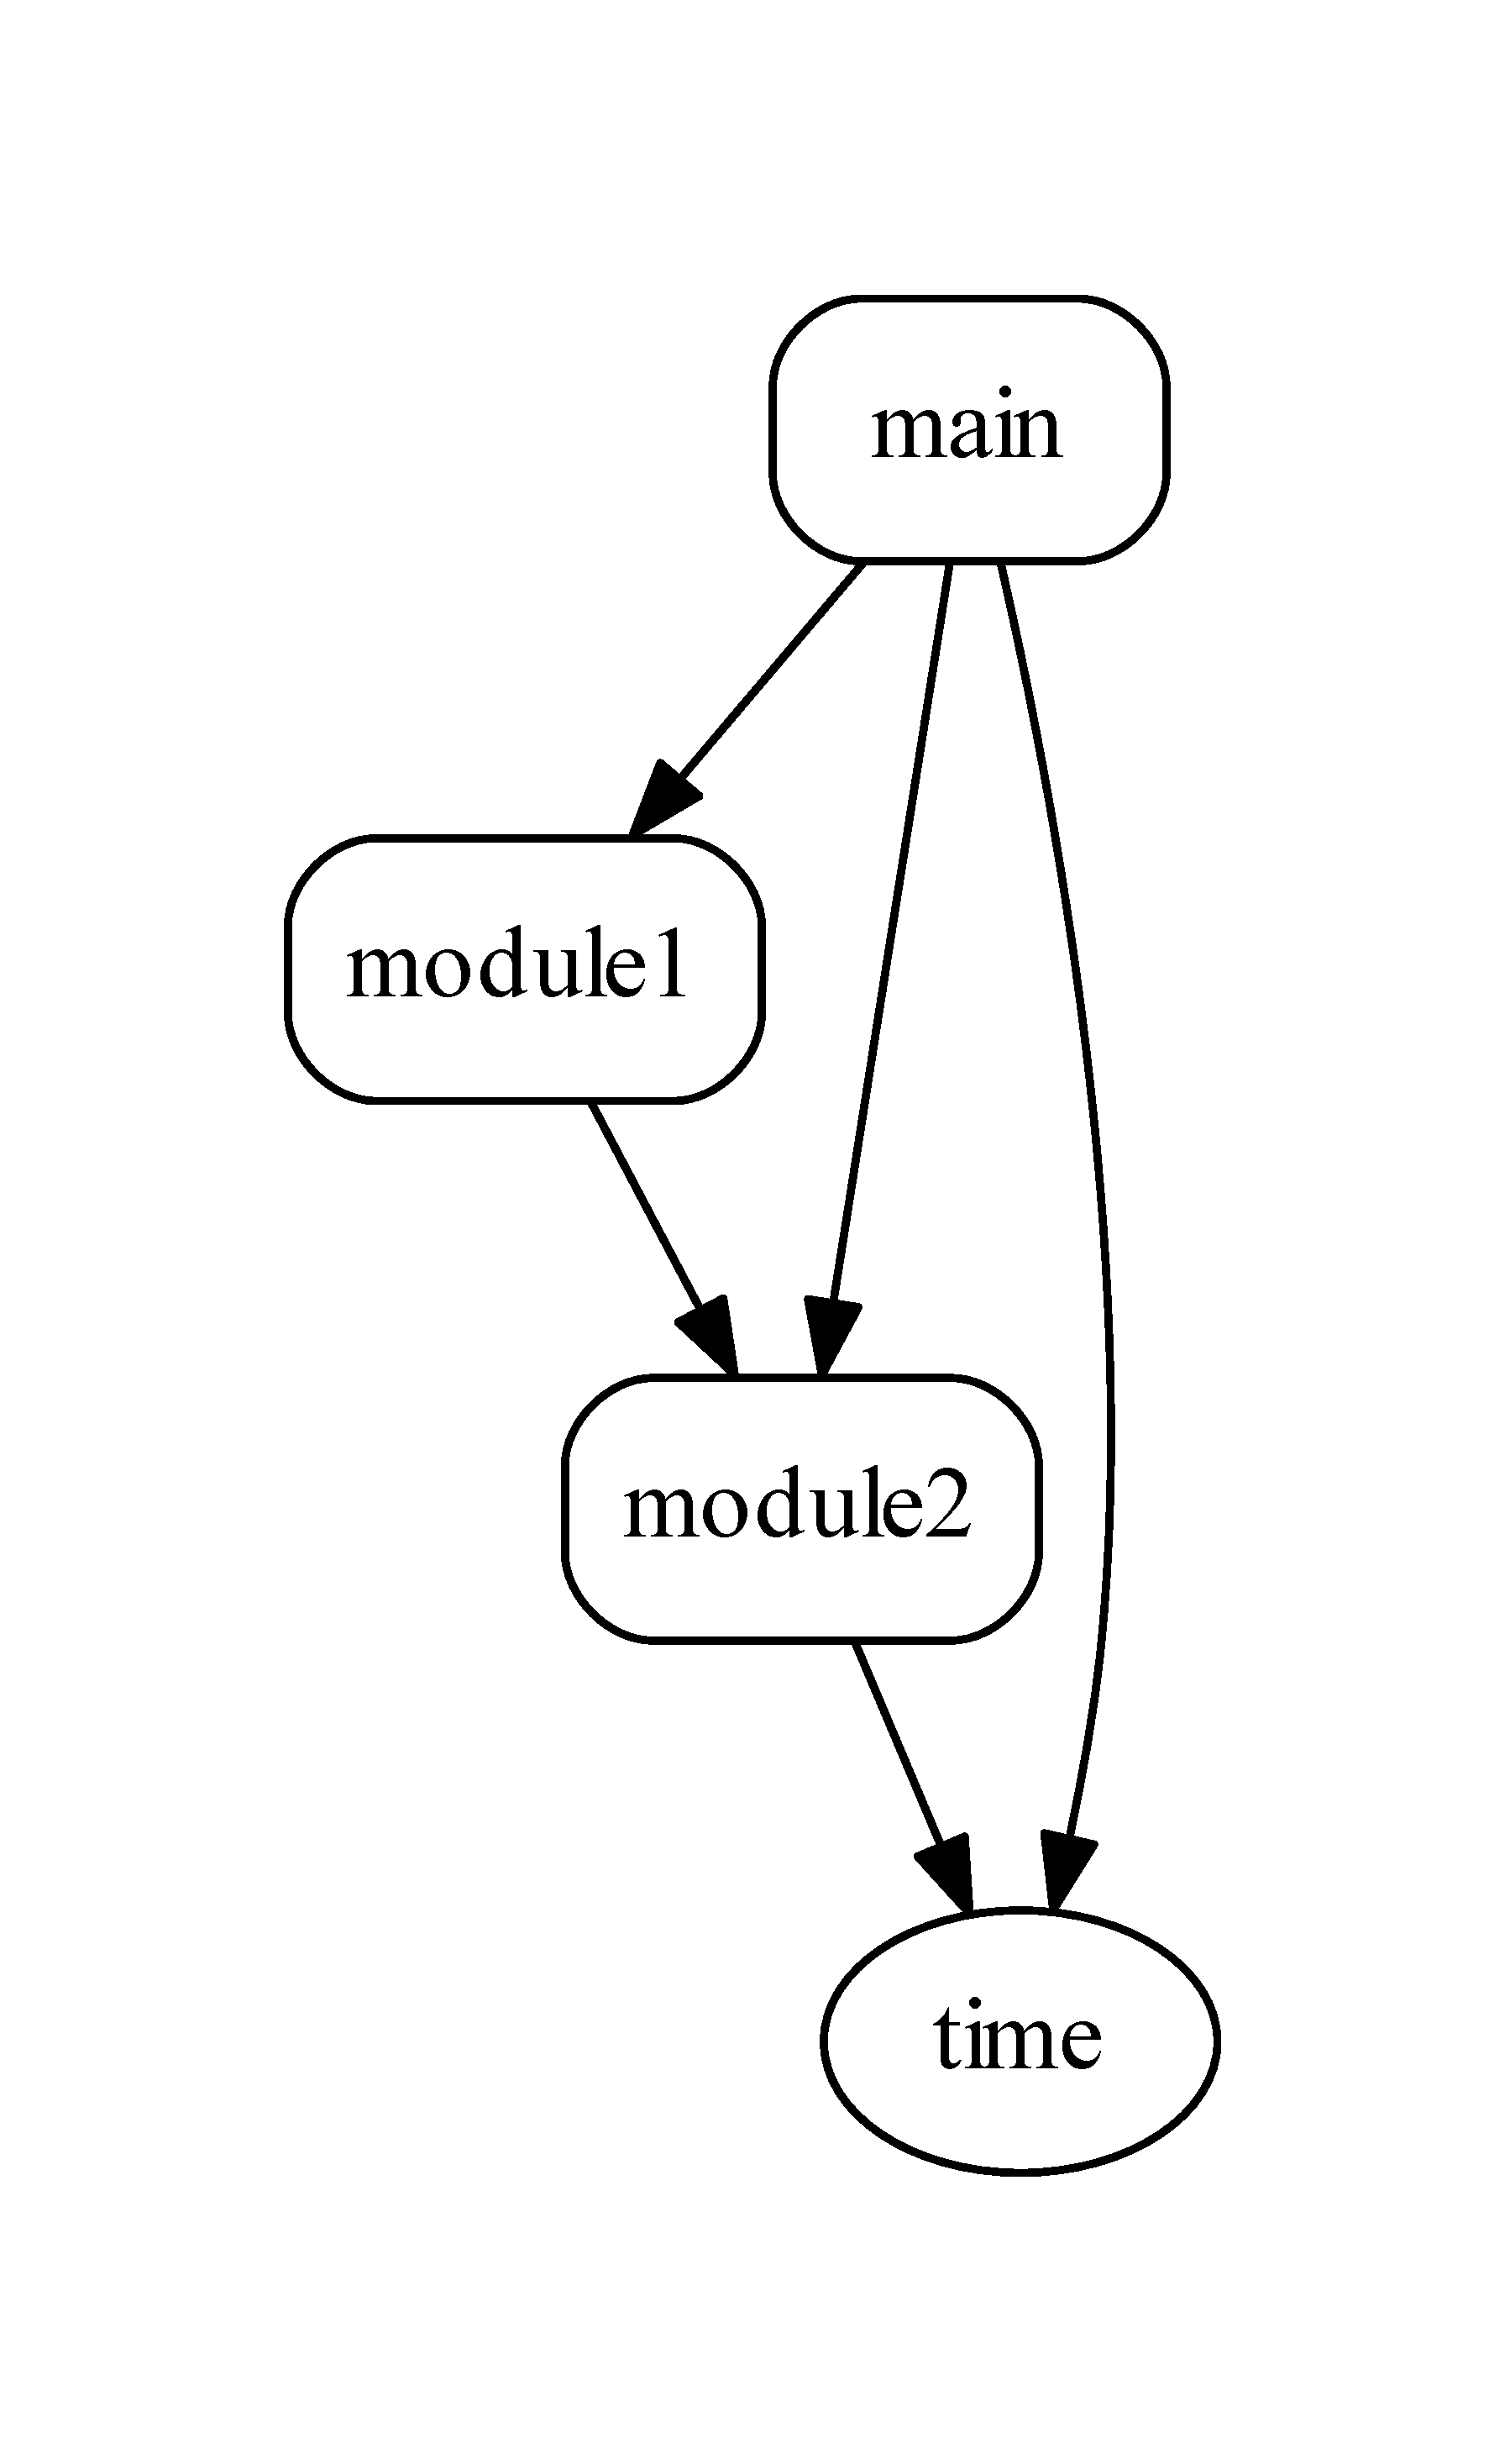
\includegraphics[width=.3\linewidth]{\home/images/Example5.pdf}
        \caption{Complete Type Graph}
    \end{center}
\end{figure}
\begin{figure}[H]
\begin{center}
    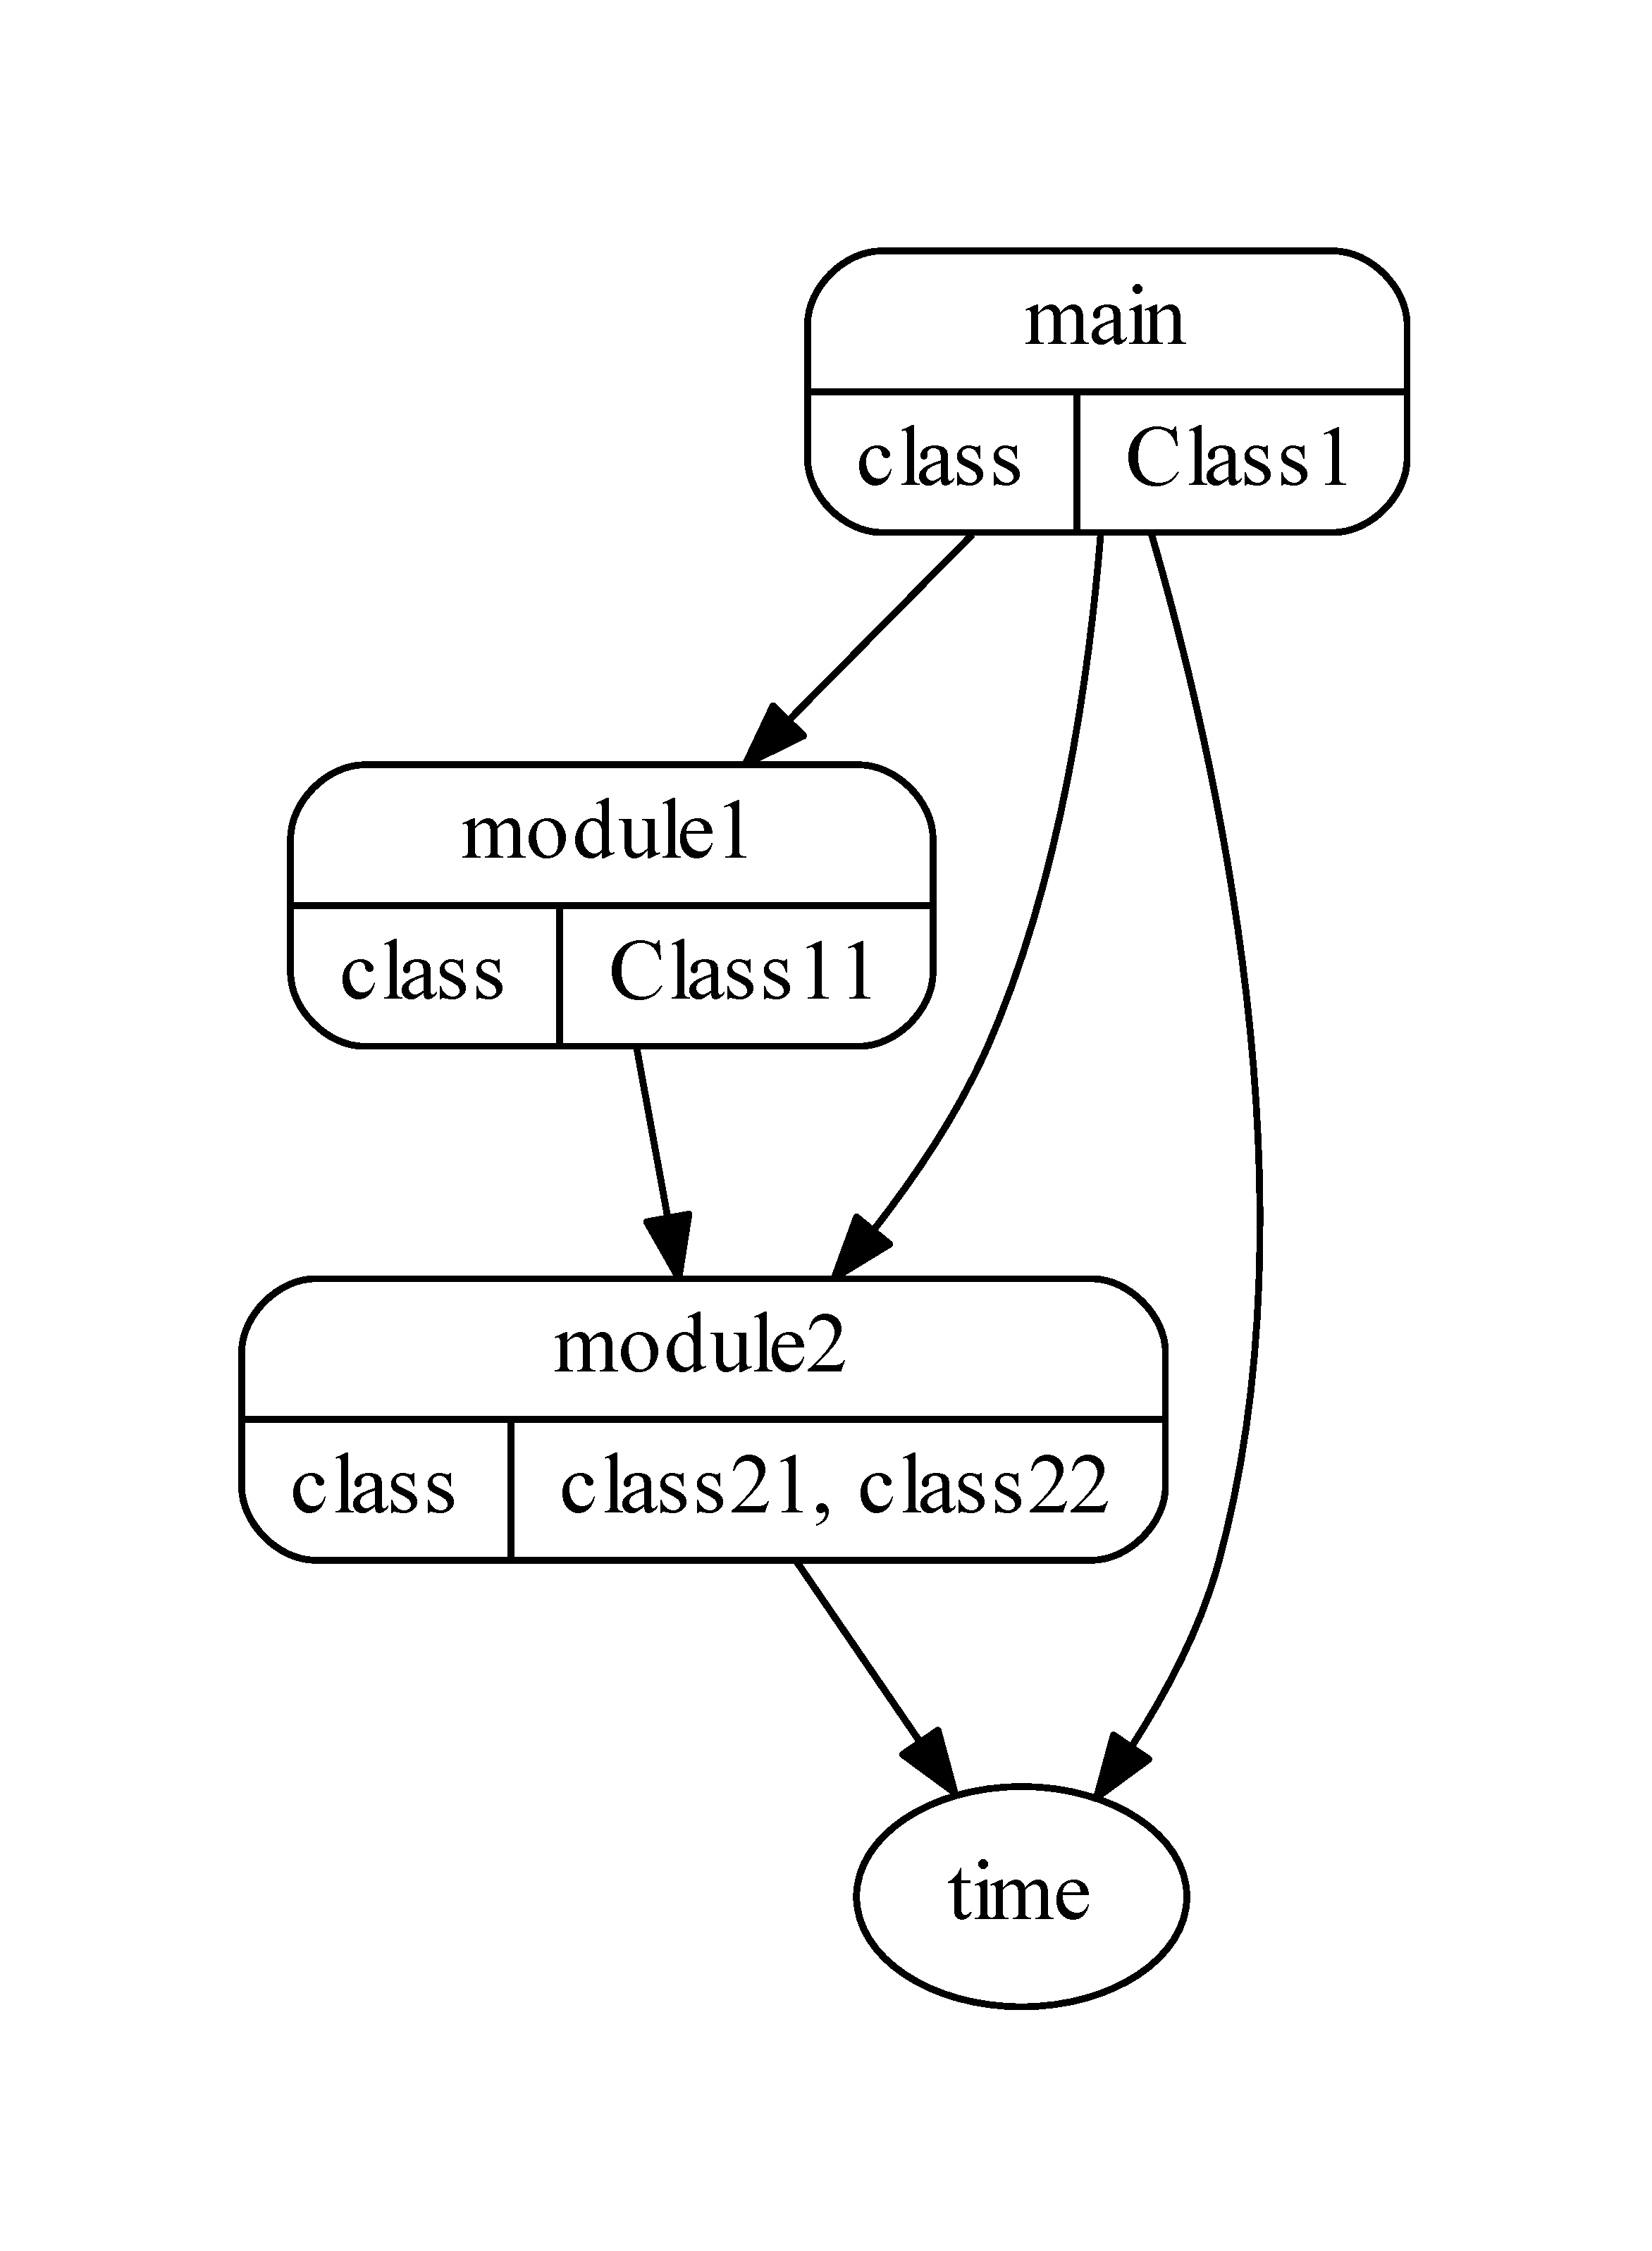
\includegraphics[width=.4\linewidth]{\home/images/Example6.pdf}
    \caption{Complete Type Graph}
\end{center}
\end{figure}